\subsubsection{Коррекция (патчинг) строки (Win32)}

Мы можем легко найти строку ``hello, world'' в исполняемом файле при помощи Hiew:

\begin{figure}[H]
\centering
\myincludegraphics{patterns/01_helloworld/hola_edit1.png}
\caption{Hiew}
\label{}
\end{figure}

Можем перевести наше сообщение на испанский язык:

\begin{figure}[H]
\centering
\myincludegraphics{patterns/01_helloworld/hola_edit2.png}
\caption{Hiew}
\label{}
\end{figure}

Испанский текст на 1 байт короче английского, так что добавляем в конце байт 0x0A (\TT{\textbackslash{}n}) и нулевой байт.

Работает.

Что если мы хотим вставить более длинное сообщение?
После оригинального текста на английском есть какие-то нулевые байты.
Трудно сказать, можно ли их перезаписывать: они могут где-то использоваться в \ac{CRT}-коде, а может и нет.
Так или иначе, вы можете их перезаписывать, только если вы действительно знаете, что делаете.

\subsubsection{Коррекция строки (Linux x64)}

\myindex{\radare}
Попробуем пропатчить исполняемый файл для Linux x64 используя \radare{}:

\lstinputlisting[caption=Сессия в \radare{}]{patterns/01_helloworld/radare.lst}

Что я здесь делаю: ищу строку \q{hello} используя команду \TT{/}, 
я затем я выставляю \emph{курсор} (\emph{seek} в терминах \radare{}) на этот адрес.
Потом я хочу удостовериться, что это действительно нужное место: \TT{px} выводит байты по этому адресу.
\TT{oo+} переключает \radare{} в режим \emph{чтения-записи}.
\TT{w} записывает ASCII-строку на месте курсора (\emph{seek}).
Нужно отметить \TT{\textbackslash{}00} в конце --- это нулевой байт.
\TT{q} заканчивает работу.

\subsubsection{Это реальная история взлома ПО}
\myindex{\SoftwareCracking}

Некое ПО обрабатывало изображения, и когда не было зарегистрированно, оно добавляло водяные знаки,
вроде ``This image was processed by evaluation version of [software name]'', поперек картинки.
Мы попробовали от балды: нашли эту строку в исполняемом файле и забили пробелами.
Водяные знаки пропали.
Технически, они продолжали добавляться.
\myindex{Qt}
При помощи соответствующих ф-ций Qt, надпись продолжала добавляться в итоговое изображение.
Но добавление пробелов не меняло само изображение...

\subsubsection{Локализация ПО во времена MS-DOS}
\myindex{MS-DOS}

Описанный способ был очень распространен для перевода ПО под MS-DOS на русский язык в 1980-е и 1990-е.
Эта техника доступна даже для тех, кто вовсе не разбирается в машинном коде и форматах исполняемых
файлов.
Новая строка не должна быть длиннее старой, потому что имеется риск затереть какую-то другую переменную
или код.
Русские слова и предложения обычно немного длиннее английских, так что \emph{локализованное} ПО содержало
массу странных акронимов и труднопонятных сокращений.

\begin{figure}[H]
\centering
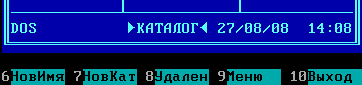
\includegraphics[width=0.5\textwidth]{patterns/01_helloworld/Norton_Commander_v5_51.png}
\caption{Русифицированный Norton Commander 5.51}
\end{figure}

Вероятно, так было и с другими языками в других странах.

\myindex{Borland Delphi}
В строках в Delphi, длина строки также должна быть поправлена, если нужно.
